\part{Hybridné modelovanie a jeho využitie v praxi}
\chapter{Hybridné modelovanie}
Úlohou modelovania procesov je získať matematický predpis na základe znalostí, ktoré o tomto procese máme~\cite{hangos:process_modelling:2001}. V závislosti od prístupu k modelovaniu, môžeme získané modely rozdeliť do viacerých skupín. Prvou skupinou sú takzvané \aps{mechanistické} modely. Tieto sú odvodené z fyzikálnych zákonov, ktoré predstavujú rôzne zákony zachovania -- bilancie, hmoty alebo energie, zákony kinetiky, termodynamiky, prestupu látky atď~\cite{bangi:chem_engineer:2020}. Takéto modely sú transparentné a ľahko pochopiteľné, pretože majú za sebou skutočnú fyzikálnu podstatu, ktorá platí pre široké spektrum prevádzkových podmienok. Nevýhodou býva, že často sú veľmi zložité a samotné modelovanie je náročné na čas. Druhú skupinu tvoria dátové modely, ktorých problematiku sme rozobrali v predchádzajúcich kapitolách. Spomenieme, že majú viacero výhod --- sú jednoduché na získanie, čím ušetríme značné množstvo času s modelovaním, často majú jednoduchšiu štruktúru, sú flexibilnejšie atď. Nevýhodou však je, že ich štruktúra nám neprezradí nič o samotnej povahe procesu. Hybridné modely tvoria tretiu skupinu a sú kombináciou mechanistických a dátových modelov, pričom využívajú výhody z obidvoch skupín, čím našli široké uplatnenie v rôznych oblastiach --- bioinžinierstvo~\cite{srivastava:hybrid_biomolecules:2020}, strojníctvo~\cite{liu:hybrid_vehicle:2020}, životné prostredie~\cite{liu:hybrid_waste_water:2019}, energetika~\cite{qian:hybrid_energy:2019} atď.

\section{Hybridné modely}
Základy hybridného modelovania položili Psichogios a Ungar v práci \aps{\textit{A hybrid neural network-first principles approach to process modeling}} z roku 1992~\cite{psichogios:hybrid_process_model:1992}. Ich cieľom bolo vytvoriť hybridný model založený na neurónovej sieti a mechanistickom modeli vsádzkového biochemického reaktora. Vo výsledku sa im podarilo zlepšiť presnosť predikcie v porovnaní so samotným mechanistickým modelom, dosiahnuť lepšiu interpoláciu a extrapoláciu na rozdiel od samotnej neurónovej siete a výrazne sa uľahčila analýza a interpretácia dát.

Treba zdôrazniť, že pri viacerých chemických, biologických a rôznych ďalších procesoch sú parametre modelu neznáme, pretože zohľadňujú napr. kinetiku konkrétnej chemickej reakcie alebo rast mikroorganizmov, ktorý je špecifický pre konkrétny druh. Ak dátový model dokáže poskytnúť tieto neznáme parametre mechanistickému modelu, tak výsledný hybridný model je vhodný aj na predikciu údajov, a tým pádom sa môže využiť na optimalizáciu procesov.
\begin{figure}
	\centering
	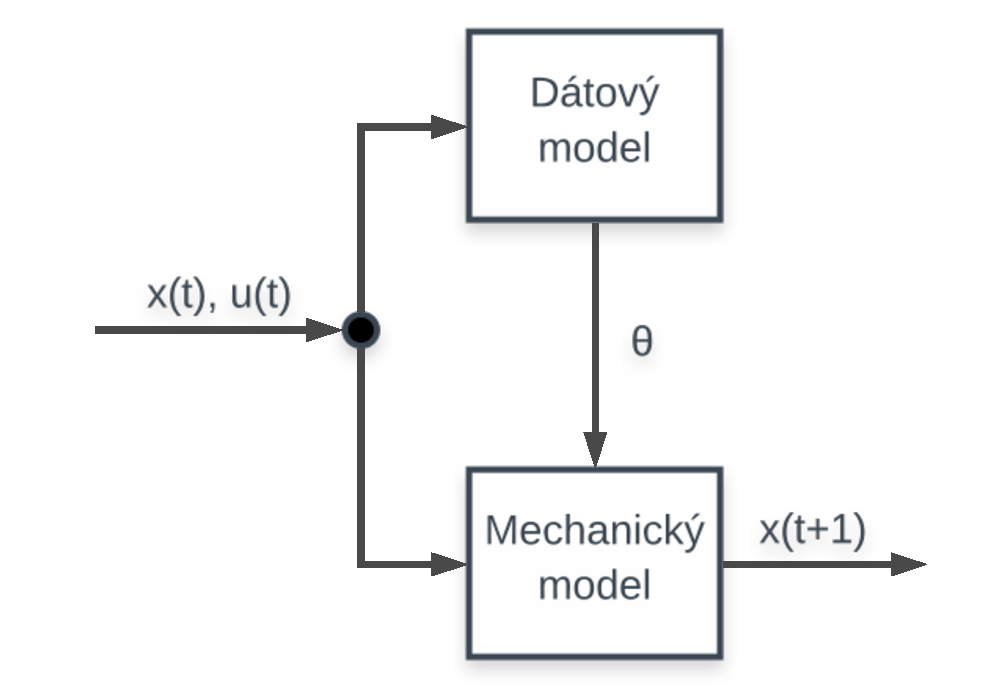
\includegraphics[width=\linewidth]{images/hybrid_model}
	\caption{Architektúra hybridných modelov - a) v sérii, b) paralelne, c) kombinácia v sérii-paralelne.}
	\label{fig:hybrid_model_general}
\end{figure} 

Existuje veľa rôznych kombinácii mechanistických a dátových modelov, ktoré vedú k ešte väčšiemu množstvu hybridných modelov, ale vo všeobecnosti by sme mohli sformulovať tri základné štruktúry hybridných modelov, ktoré sú zobrazené na Obr. \ref{fig:hybrid_model_general}.

\textbf{Zapojenie v sérii.} Takáto štruktúra hybridných modelov sa využíva na odhad neznámych  a časovo-premenných kinetických parametrov $ \theta $~\cite{bhutani:hybrid_modelling_opt:2006}.\newline
\textbf{Paralelné zapojenie.} Zatiaľ čo nominálny mechanistický model zachytáva správanie systému, dátová časť koriguje rozdiely $ \Delta $ medzi skutočným zariadením a mechanistickým modelom. Dátový model natrénovaný na týchto rozdieloch, kompenzuje chyby, ktoré vyplývajú z bežných variácií procesu a nelineárnej komplexnej kinetiky~\cite{bhutani:hybrid_modelling_opt:2006}.\newline
\textbf{Kombinovaný prístup -- sériovo-paralelné zapojenie.} V tomto prípade daná architektúra obsahuje dva dátové modely -- jeden, ktorý odhaduje neznáme parametre systému $ \theta $ (v sérii) a druhý, ktorý upravuje výstupy z mechanistického modelu o rozdiel oproti skutočnému zariadeniu (paralelne). 
